\documentclass[11pt, a4paper, twoside]{article}   	% use "amsart" instead of "article" for AMSLaTeX format

\usepackage{geometry}                		% See geometry.pdf to learn the layout options. There are lots.
\usepackage{pdfpages}
\usepackage{caption}
\usepackage{minted}
\usepackage[german]{babel}			% this end the next are needed for german umlaute
\usepackage[utf8]{inputenc}
\usepackage{color}
\usepackage{graphicx}
\usepackage{titlesec}
\usepackage{fancyhdr}
\usepackage{lastpage}
\usepackage{hyperref}
% http://www.artofproblemsolving.com/wiki/index.php/LaTeX:Symbols#Operators
% =============================================
% Layout & Colors
% =============================================
\geometry{
   a4paper,
   total={210mm,297mm},
   left=20mm,
   right=20mm,
   top=20mm,
   bottom=30mm
 }	

\definecolor{myred}{rgb}{0.8,0,0}
\definecolor{mygreen}{rgb}{0,0.6,0}
\definecolor{mygray}{rgb}{0.5,0.5,0.5}
\definecolor{mymauve}{rgb}{0.58,0,0.82}

\setcounter{secnumdepth}{4}


% the default java directory structure and the main packages
\newcommand{\srcDir}{/src/main/java}
% =============================================
% Code Settings
% =============================================
\newenvironment{code}{\captionsetup{type=listing}}{}
\newmintedfile[javaSourceFile]{java}{
	linenos=true, 
	frame=single, 
	breaklines=true, 
	tabsize=2,
	numbersep=5pt,
	xleftmargin=10pt,
	baselinestretch=1,
	fontsize=\footnotesize
}
\newmintinline[inlineJava]{java}{}
\newminted[javaSource]{java}{
	breaklines=true, 
	tabsize=2,
	autogobble=true,
	breakautoindent=false
}
\newmintedfile[xmlSourceFile]{xml}{
	linenos=true, 
	frame=single, 
	breaklines=true, 
	tabsize=2,
	numbersep=5pt,
	xleftmargin=10pt,
	baselinestretch=1,
	fontsize=\footnotesize
}
\newmintedfile[propertiesFile]{properties}{
	linenos=true, 
	frame=single, 
	breaklines=true, 
	tabsize=2,
	numbersep=5pt,
	xleftmargin=10pt,
	baselinestretch=1,
	fontsize=\footnotesize
}
\newmintedfile[sqlFile]{sql}{
	linenos=true, 
	frame=single, 
	breaklines=true, 
	tabsize=2,
	numbersep=5pt,
	xleftmargin=10pt,
	baselinestretch=1,
	fontsize=\footnotesize
}
% =============================================
% Page Style, Footers & Headers, Title
% =============================================
\title{Übung 3}
\author{Thomas Herzog}

\lhead{Übung 3}
\chead{}
\rhead{
\includegraphics[scale=0.10]{FHO_Logo_Students.jpg}}

\lfoot{S1310307011}
\cfoot{}
\rfoot{ \thepage / \pageref{LastPage} }
\renewcommand{\footrulewidth}{0.4pt}
% =============================================
% D O C U M E N T     C O N T E N T
% =============================================
\pagestyle{fancy}
\begin{document}
\setlength{\headheight}{15mm}
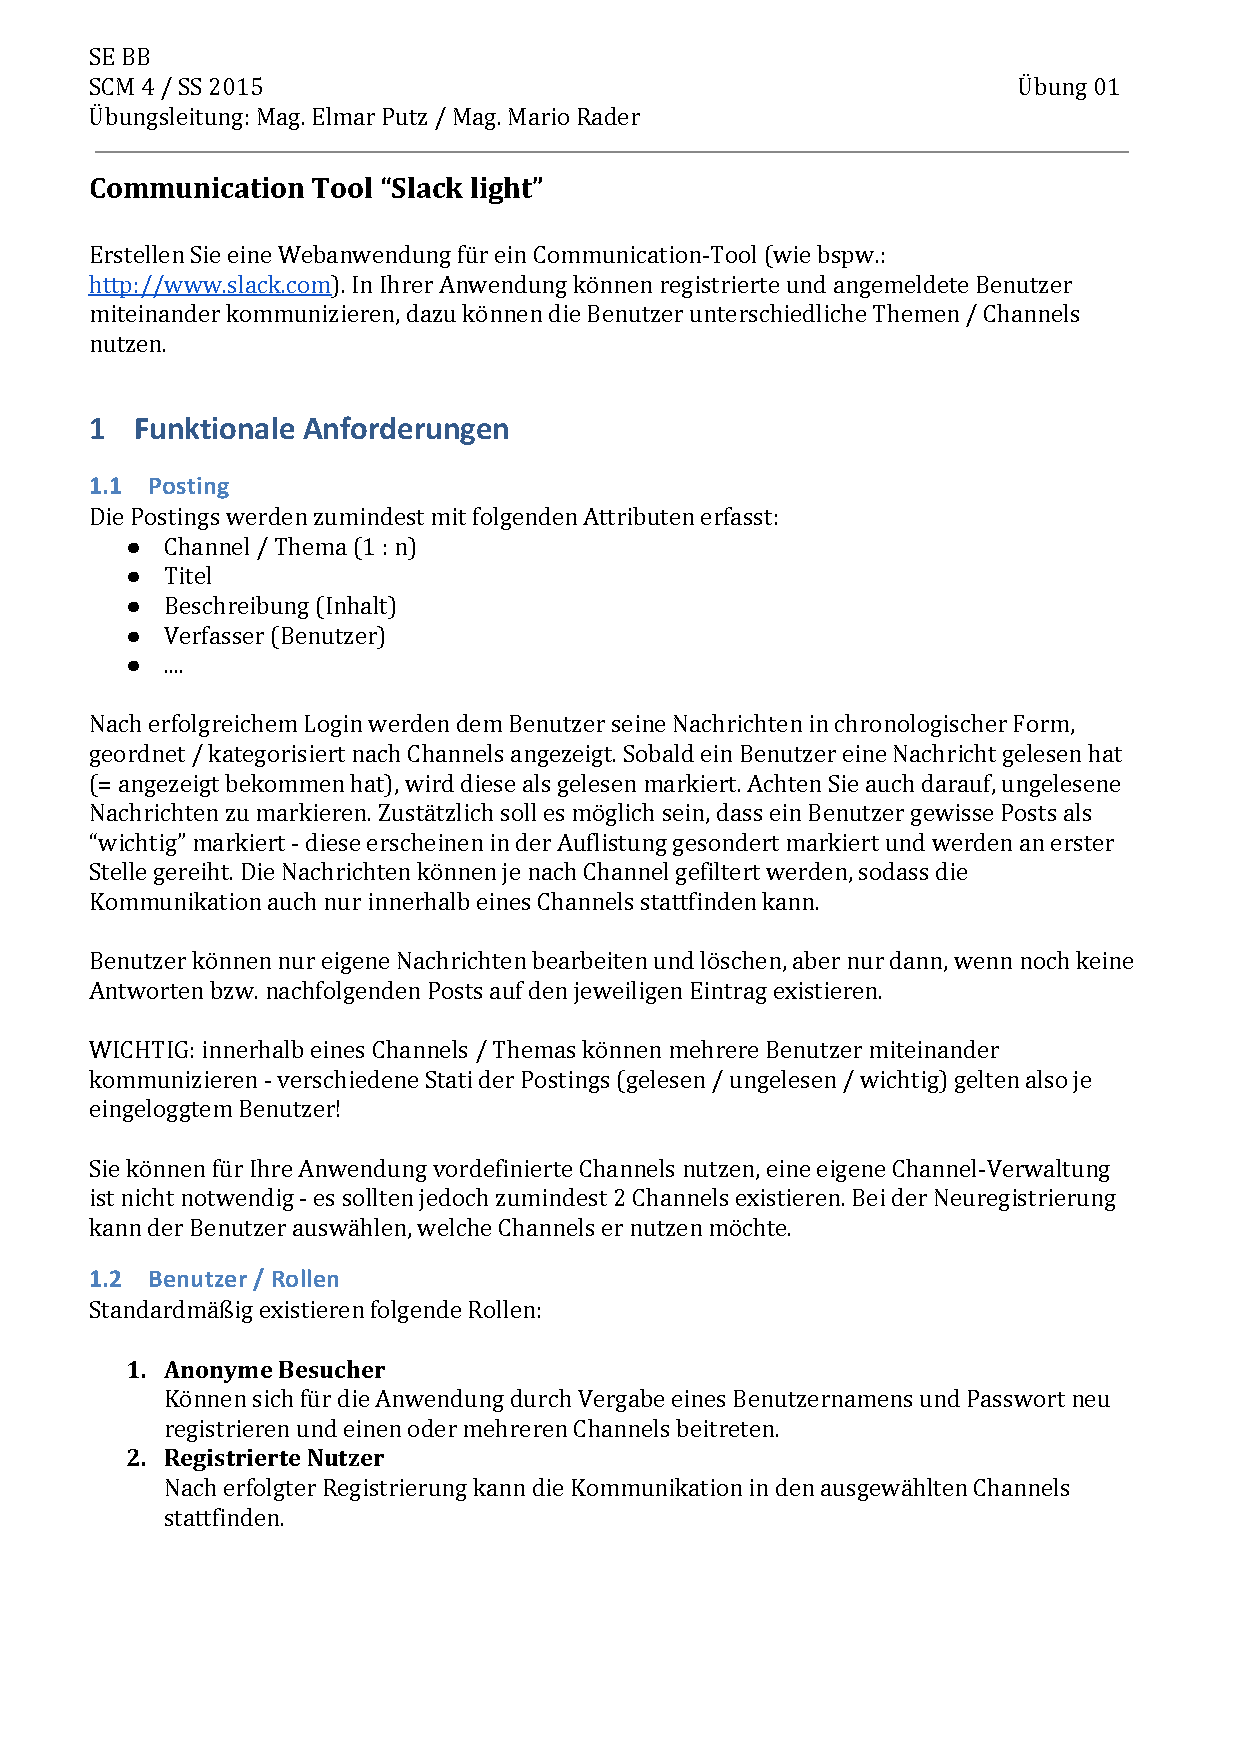
\includepdf[pages={1,2,3}]{scm4-2015-uebung01-communication-list.pdf}
{\color{myred}
	\section
		{Kommunikationstool 'Slack Light'}
}

% =============================================
% Idea section
% =============================================
\subsection{Datenbank}
Folgende Abbildung zeigt das ER Diagramm des Datenmodells für das Kommunikationstool "Slack light". \
\begin{figure}[h]
	\centering
	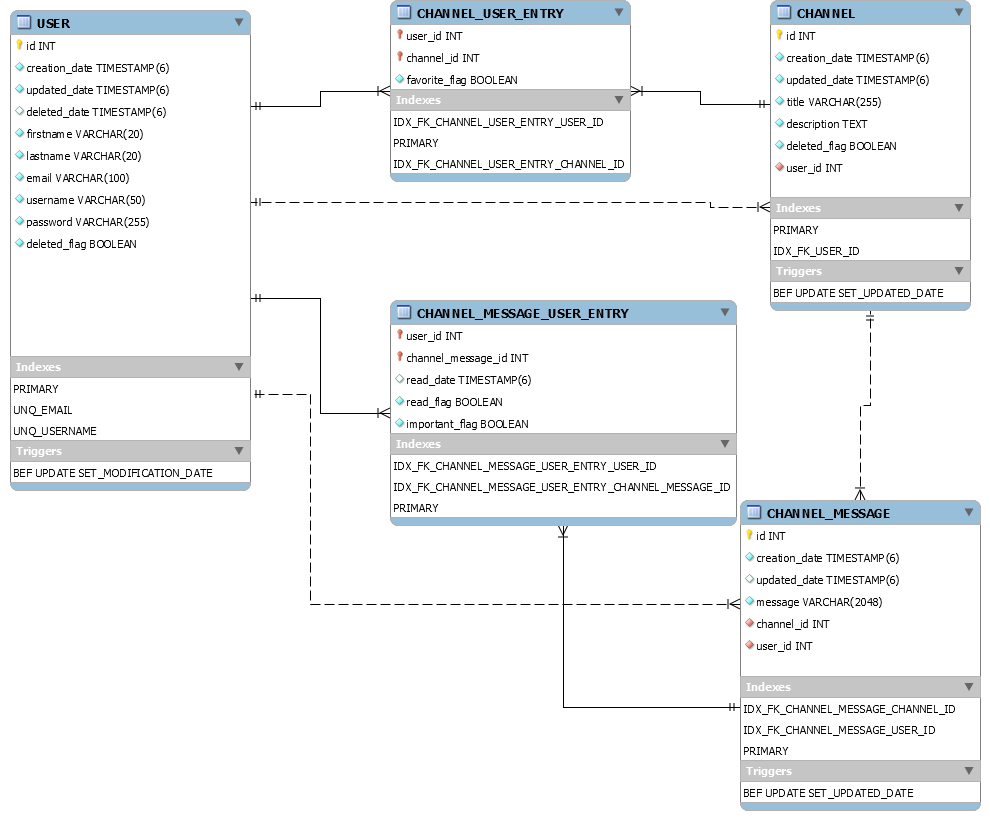
\includegraphics[scale=0.5]{images/er-model.PNG}
	\caption
	{ER-Modell}
\end{figure}

\newpage
\subsection{Applikationsarchitektur}
Folgender Abschnitt beschreibt die Architektur der Applikation.\\
Die Applikation ist in zwei Haupt PHP Dateien aufgeteilt über die alle Request gehandelt werden:
\begin{enumerate}
	\item \textbf{index.php:} \\
	All offenen Ressourcen wie Login und Registrierung 
	\item \textbf{start.php:} \\
	Alle geschützten Ressourcen, die einen Login erfordern.
\end{enumerate}
Diese Dateien sowie alle *.css, *.js Dateien sowie Images sind in einem public Verzeichnis zusammengefasst und können ohne Zugriffskontrolle abgerufen werden.\\
Alle anderen angezeigten Seiten werden über das Templating Tool \textbf{Twig} generiert und werden über die beiden PHP Dateien index.php oder start.php and den Client übermittelt. Dadurch ist kein direkter Zugriff auf diese Dateien möglich. \\\\
Folgende Abbildung illustriert den Aufbau der Applikation beziehungsweise den Ablauf eines Requests. \\
\\
TODO: Add image regarding aplication structure or request handling 

\end{document}  